\documentclass{article}
% Language setting
% Replace `english' with e.g. `spanish' to change the document language
\usepackage[english]{babel}

% Set page size and margins
% Replace `letterpaper' with`a4paper' for UK/EU standard size
\usepackage[letterpaper,top=2cm,bottom=2cm,left=3cm,right=3cm,marginparwidth=1.75cm]{geometry}

% Useful packages
\usepackage{amsmath}
\usepackage{graphicx}
\usepackage{caption}

\usepackage[colorlinks=true, allcolors=blue]{hyperref}

\title{Imágenes Servicio Social}
\author{Robles Gómez Mariano}

\begin{document}
	\maketitle


\begin{figure}
	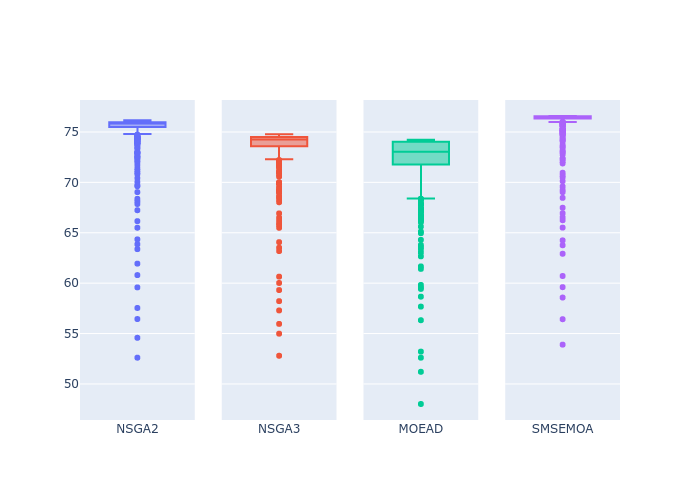
\includegraphics[width=0.3\textwidth]{wfg3_hv_3_bp.png}
	\caption[width=0.3]{Diagrama de caja del problema wfg3 con indicador hv con 3 objetivos.}
\end{figure}
\begin{figure}
	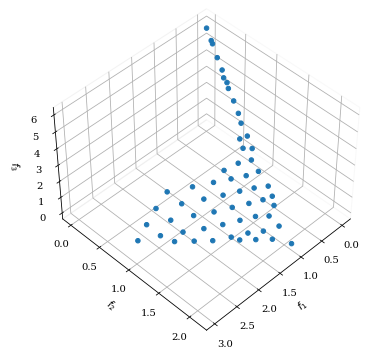
\includegraphics[width=0.3\textwidth]{NSGA3_wfg3_igdp_3_fp.png}
	\caption{Aproximación al frente de pareto del problema wfg3 con indicador igdp usando algoritmoNSGA3 con 3 objetivos.}
\end{figure}
\begin{figure}
	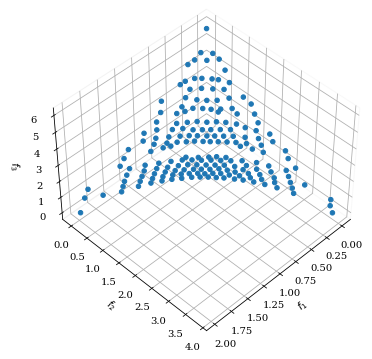
\includegraphics[width=0.3\textwidth]{NSGA3_wfg2_hv_3_fp.png}
	\caption{Aproximación al frente de pareto del problema wfg2 con indicador hv usando algoritmoNSGA3 con 3 objetivos.}
\end{figure}
\clearpage
\begin{figure}
	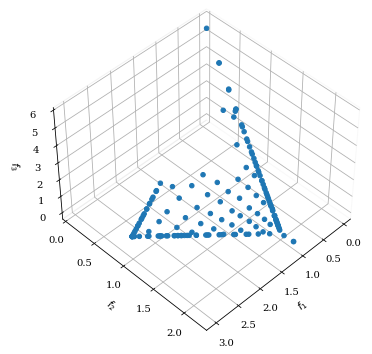
\includegraphics[width=0.3\textwidth]{MOEAD_wfg3_igdp_3_fp.png}
	\caption{Aproximación al frente de pareto del problema wfg3 con indicador igdp usando algoritmoMOEAD con 3 objetivos.}
\end{figure}
\begin{figure}
	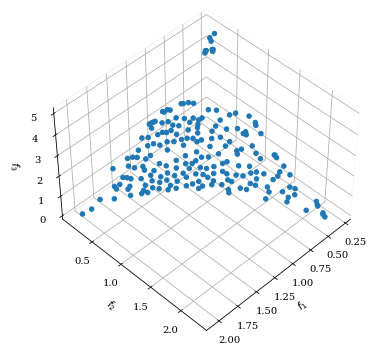
\includegraphics[width=0.3\textwidth]{SMSEMOA_wfg1_Tiempo_3_fp.png}
	\caption{Aproximación al frente de pareto del problema wfg1 con indicador Tiempo usando algoritmoSMSEMOA con 3 objetivos.}
\end{figure}
\begin{figure}
	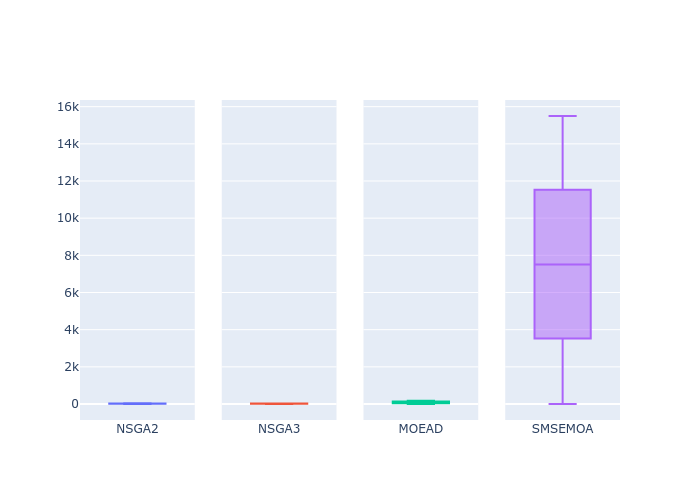
\includegraphics[width=0.3\textwidth]{wfg3_Tiempo_3_bp.png}
	\caption{Diagrama de caja del problema wfg3 con indicador Tiempo con 3 objetivos.}
\end{figure}
\clearpage
\begin{figure}
	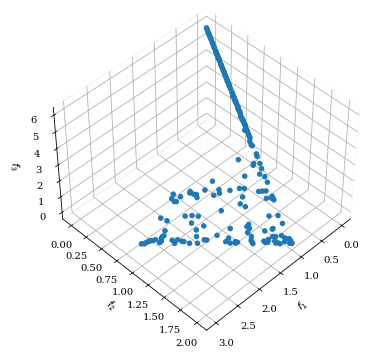
\includegraphics[width=0.3\textwidth]{NSGA2_wfg3_igdp_3_fp.png}
	\caption{Aproximación al frente de pareto del problema wfg3 con indicador igdp usando algoritmoNSGA2 con 3 objetivos.}
\end{figure}
\begin{figure}
	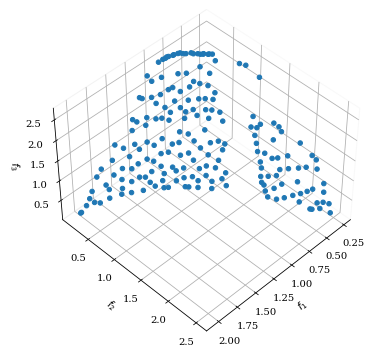
\includegraphics[width=0.3\textwidth]{SMSEMOA_wfg1_hv_3_fp.png}
	\caption{Aproximación al frente de pareto del problema wfg1 con indicador hv usando algoritmoSMSEMOA con 3 objetivos.}
\end{figure}
\begin{figure}
	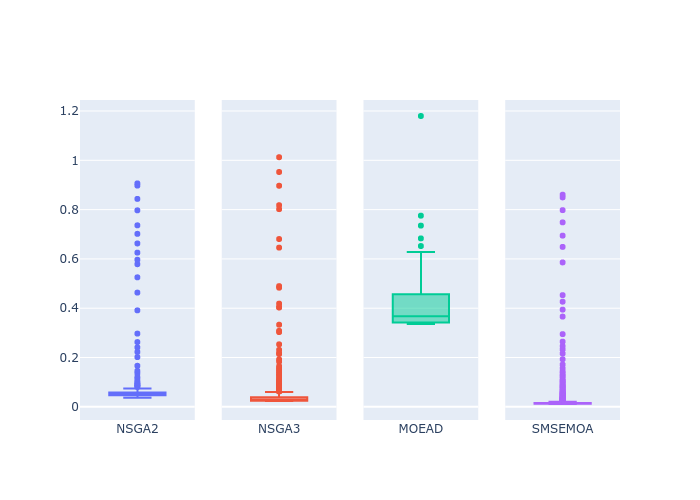
\includegraphics[width=0.3\textwidth]{wfg2_igdp_3_bp.png}
	\caption{Diagrama de caja del problema wfg2 con indicador igdp con 3 objetivos.}
\end{figure}
\clearpage
\begin{figure}
	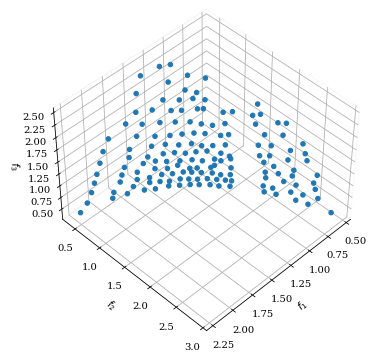
\includegraphics[width=0.3\textwidth]{NSGA3_wfg1_hv_3_fp.png}
	\caption{Aproximación al frente de pareto del problema wfg1 con indicador hv usando algoritmoNSGA3 con 3 objetivos.}
\end{figure}
\begin{figure}
	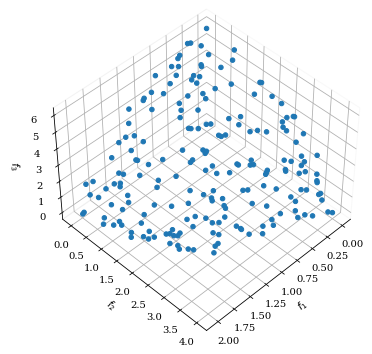
\includegraphics[width=0.3\textwidth]{NSGA2_wfg4_igdp_3_fp.png}
	\caption{Aproximación al frente de pareto del problema wfg4 con indicador igdp usando algoritmoNSGA2 con 3 objetivos.}
\end{figure}
\begin{figure}
	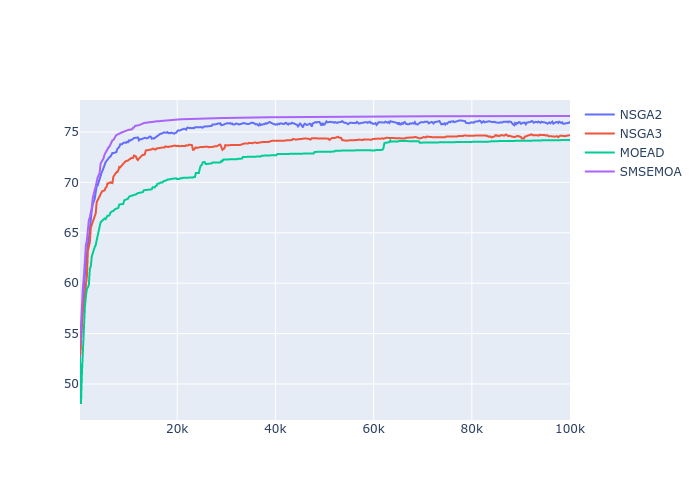
\includegraphics[width=0.3\textwidth]{wfg3_hv_3_gc.png}
	\caption{Grafico de convergencia del problema wfg3 con indicador hv con 3 objetivos.}
\end{figure}
\clearpage
\begin{figure}
	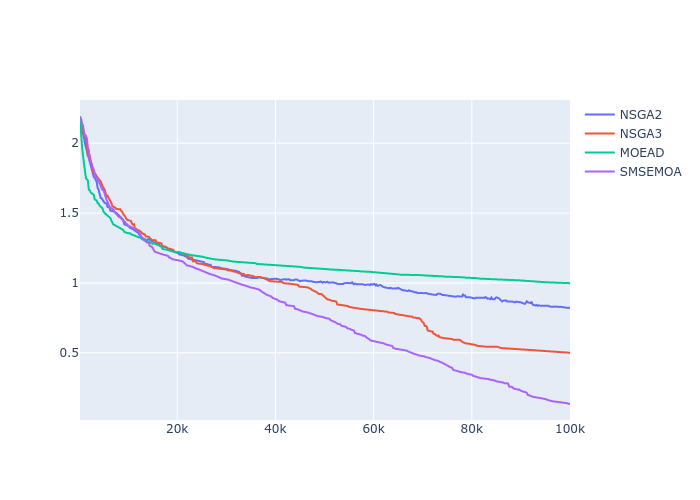
\includegraphics[width=0.3\textwidth]{wfg1_igdp_3_gc.png}
	\caption{Grafico de convergencia del problema wfg1 con indicador igdp con 3 objetivos.}
\end{figure}
\begin{figure}
	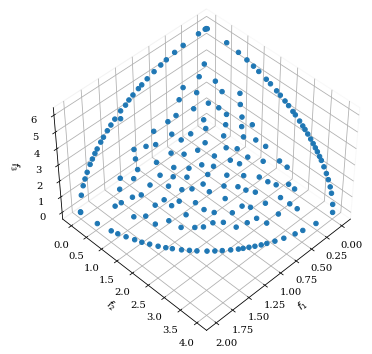
\includegraphics[width=0.3\textwidth]{SMSEMOA_wfg4_igdp_3_fp.png}
	\caption{Aproximación al frente de pareto del problema wfg4 con indicador igdp usando algoritmoSMSEMOA con 3 objetivos.}
\end{figure}
\begin{figure}
	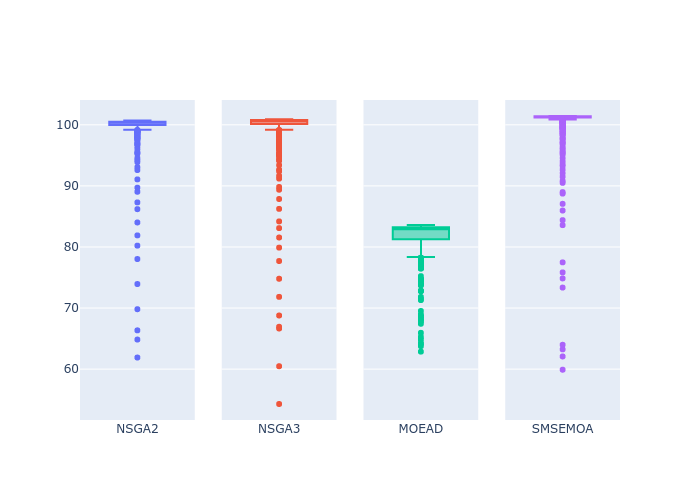
\includegraphics[width=0.3\textwidth]{wfg2_hv_3_bp.png}
	\caption{Diagrama de caja del problema wfg2 con indicador hv con 3 objetivos.}
\end{figure}
\clearpage
\begin{figure}
	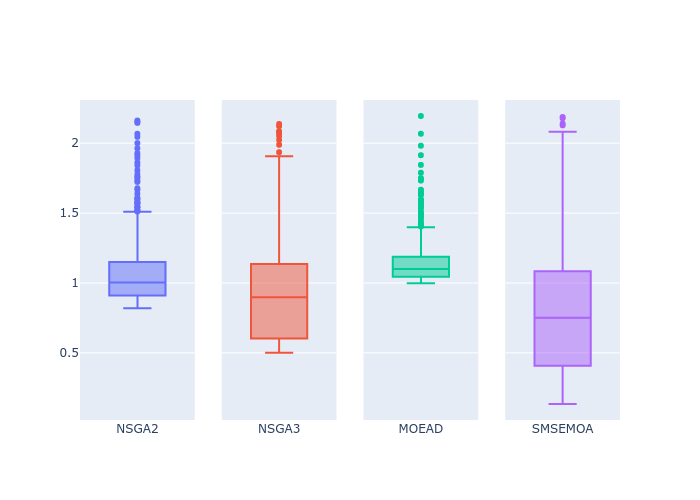
\includegraphics[width=0.3\textwidth]{wfg1_igdp_3_bp.png}
	\caption{Diagrama de caja del problema wfg1 con indicador igdp con 3 objetivos.}
\end{figure}
\begin{figure}
	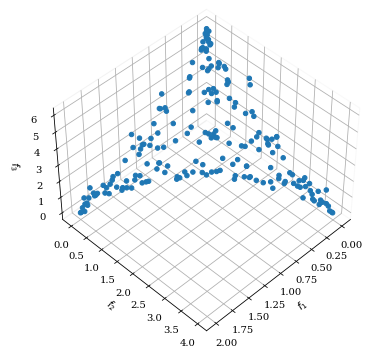
\includegraphics[width=0.3\textwidth]{NSGA2_wfg2_Tiempo_3_fp.png}
	\caption{Aproximación al frente de pareto del problema wfg2 con indicador Tiempo usando algoritmoNSGA2 con 3 objetivos.}
\end{figure}
\begin{figure}
	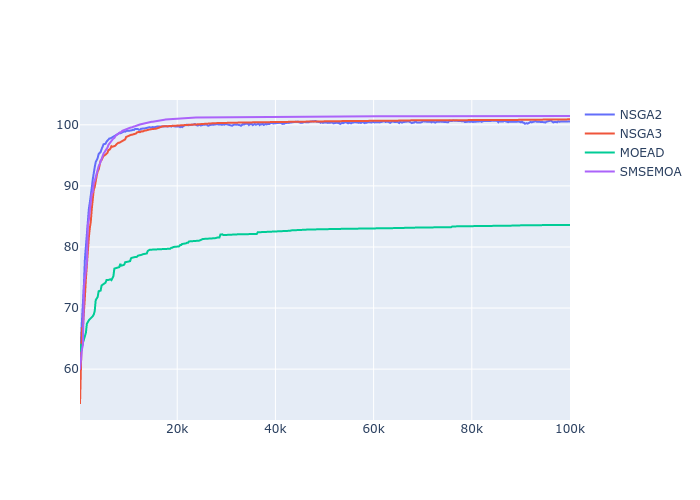
\includegraphics[width=0.3\textwidth]{wfg2_hv_3_gc.png}
	\caption{Grafico de convergencia del problema wfg2 con indicador hv con 3 objetivos.}
\end{figure}
\clearpage
\begin{figure}
	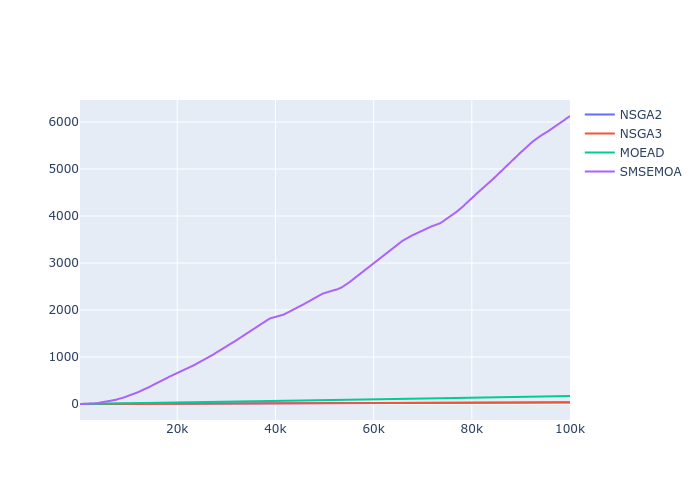
\includegraphics[width=0.3\textwidth]{wfg1_Tiempo_3_gc.png}
	\caption{Grafico de convergencia del problema wfg1 con indicador Tiempo con 3 objetivos.}
\end{figure}
\begin{figure}
	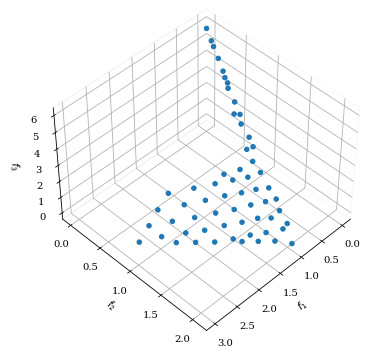
\includegraphics[width=0.3\textwidth]{NSGA3_wfg3_hv_3_fp.png}
	\caption{Aproximación al frente de pareto del problema wfg3 con indicador hv usando algoritmoNSGA3 con 3 objetivos.}
\end{figure}
\begin{figure}
	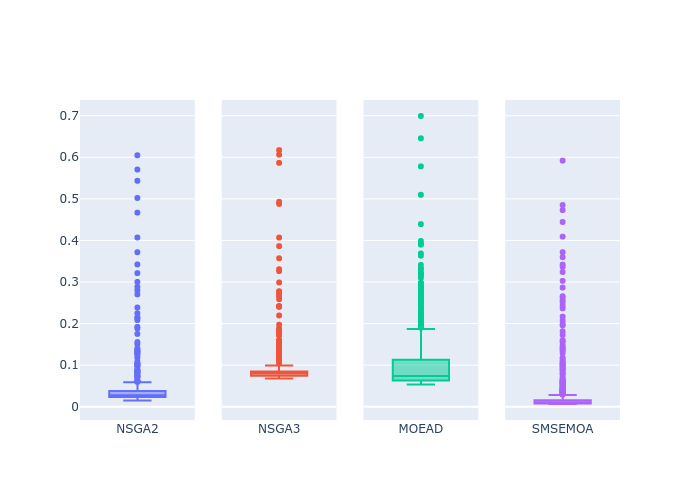
\includegraphics[width=0.3\textwidth]{wfg3_igdp_3_bp.png}
	\caption{Diagrama de caja del problema wfg3 con indicador igdp con 3 objetivos.}
\end{figure}
\clearpage
\begin{figure}
	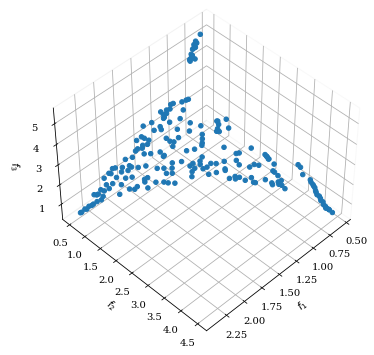
\includegraphics[width=0.3\textwidth]{NSGA2_wfg1_Tiempo_3_fp.png}
	\caption{Aproximación al frente de pareto del problema wfg1 con indicador Tiempo usando algoritmoNSGA2 con 3 objetivos.}
\end{figure}
\begin{figure}
	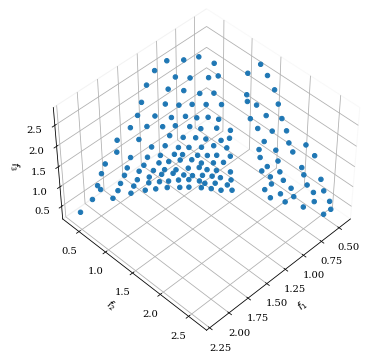
\includegraphics[width=0.3\textwidth]{NSGA3_wfg1_Tiempo_3_fp.png}
	\caption{Aproximación al frente de pareto del problema wfg1 con indicador Tiempo usando algoritmoNSGA3 con 3 objetivos.}
\end{figure}
\begin{figure}
	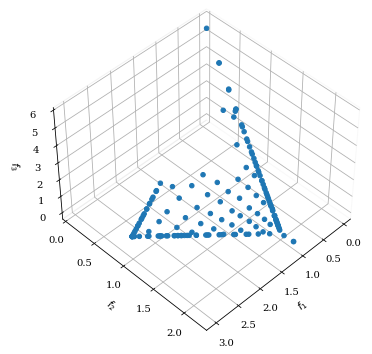
\includegraphics[width=0.3\textwidth]{MOEAD_wfg3_hv_3_fp.png}
	\caption{Aproximación al frente de pareto del problema wfg3 con indicador hv usando algoritmoMOEAD con 3 objetivos.}
\end{figure}
\clearpage
\begin{figure}
	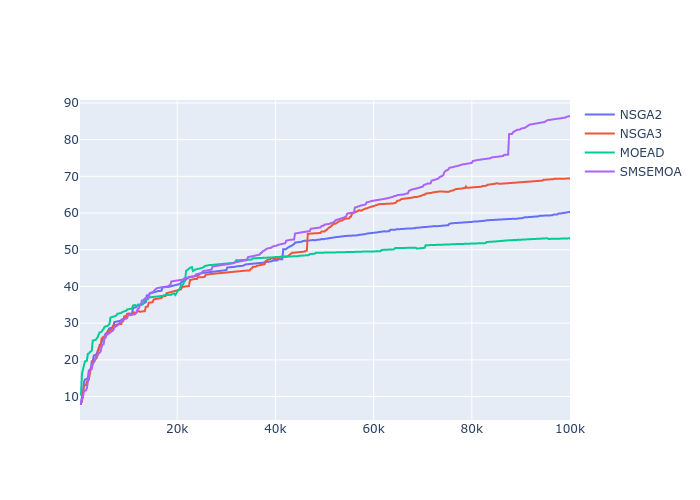
\includegraphics[width=0.3\textwidth]{wfg1_hv_3_gc.png}
	\caption{Grafico de convergencia del problema wfg1 con indicador hv con 3 objetivos.}
\end{figure}
\begin{figure}
	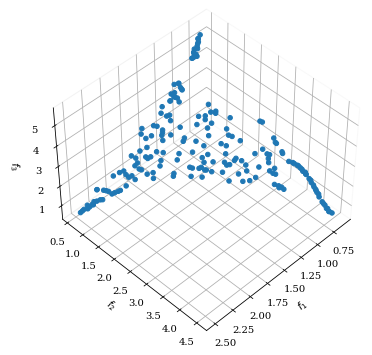
\includegraphics[width=0.3\textwidth]{NSGA2_wfg1_igdp_3_fp.png}
	\caption{Aproximación al frente de pareto del problema wfg1 con indicador igdp usando algoritmoNSGA2 con 3 objetivos.}
\end{figure}
\begin{figure}
	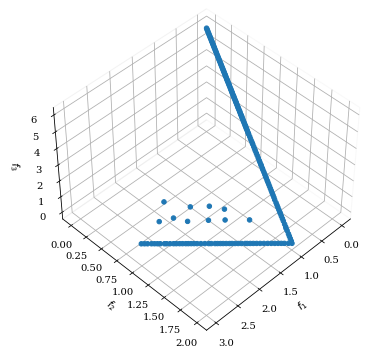
\includegraphics[width=0.3\textwidth]{SMSEMOA_wfg3_Tiempo_3_fp.png}
	\caption{Aproximación al frente de pareto del problema wfg3 con indicador Tiempo usando algoritmoSMSEMOA con 3 objetivos.}
\end{figure}
\clearpage
\begin{figure}
	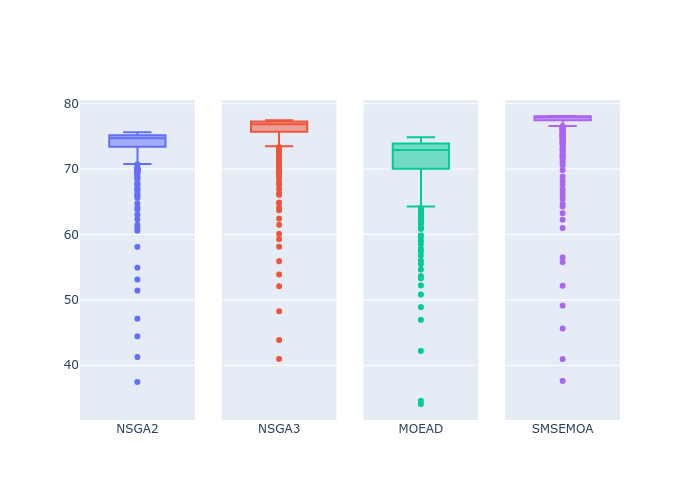
\includegraphics[width=0.3\textwidth]{wfg4_hv_3_bp.png}
	\caption{Diagrama de caja del problema wfg4 con indicador hv con 3 objetivos.}
\end{figure}
\begin{figure}
	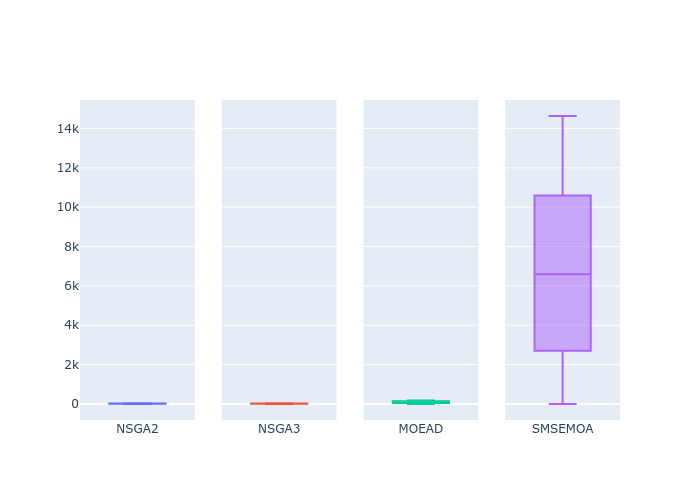
\includegraphics[width=0.3\textwidth]{wfg2_Tiempo_3_bp.png}
	\caption{Diagrama de caja del problema wfg2 con indicador Tiempo con 3 objetivos.}
\end{figure}
\begin{figure}
	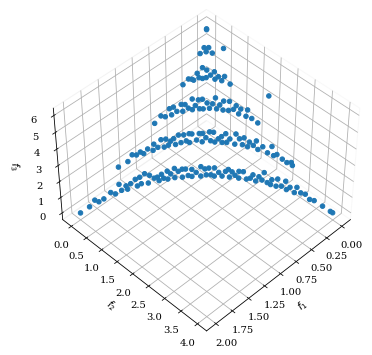
\includegraphics[width=0.3\textwidth]{SMSEMOA_wfg2_igdp_3_fp.png}
	\caption{Aproximación al frente de pareto del problema wfg2 con indicador igdp usando algoritmoSMSEMOA con 3 objetivos.}
\end{figure}
\clearpage
\begin{figure}
	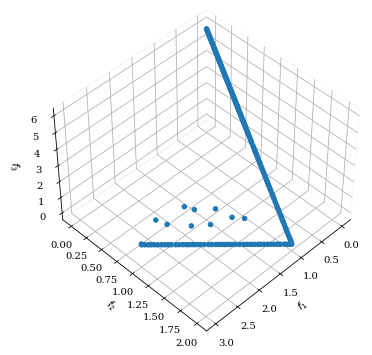
\includegraphics[width=0.3\textwidth]{SMSEMOA_wfg3_hv_3_fp.png}
	\caption{Aproximación al frente de pareto del problema wfg3 con indicador hv usando algoritmoSMSEMOA con 3 objetivos.}
\end{figure}
\begin{figure}
	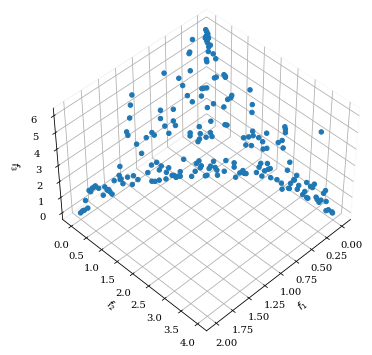
\includegraphics[width=0.3\textwidth]{NSGA2_wfg2_hv_3_fp.png}
	\caption{Aproximación al frente de pareto del problema wfg2 con indicador hv usando algoritmoNSGA2 con 3 objetivos.}
\end{figure}
\begin{figure}
	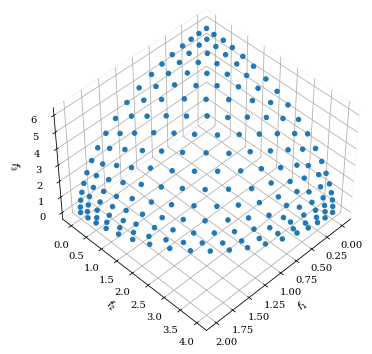
\includegraphics[width=0.3\textwidth]{NSGA3_wfg4_Tiempo_3_fp.png}
	\caption{Aproximación al frente de pareto del problema wfg4 con indicador Tiempo usando algoritmoNSGA3 con 3 objetivos.}
\end{figure}
\clearpage
\begin{figure}
	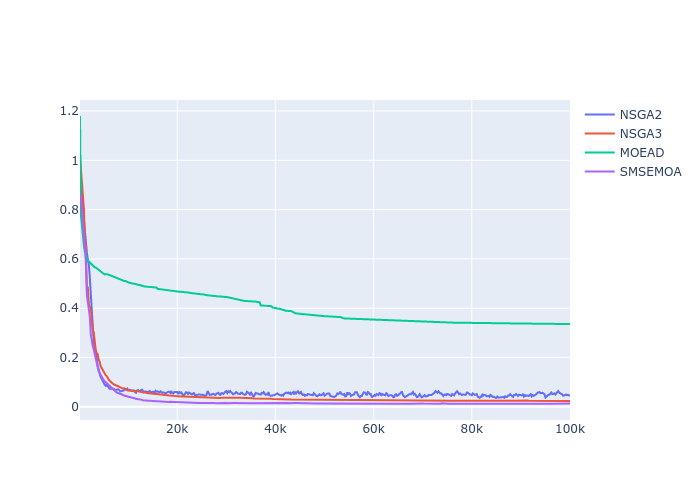
\includegraphics[width=0.3\textwidth]{wfg2_igdp_3_gc.png}
	\caption{Grafico de convergencia del problema wfg2 con indicador igdp con 3 objetivos.}
\end{figure}
\begin{figure}
	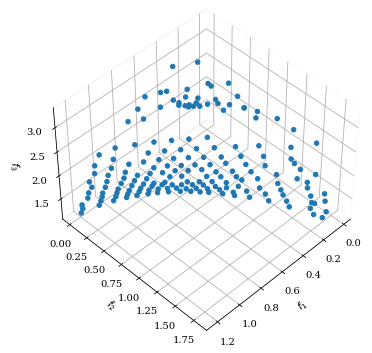
\includegraphics[width=0.3\textwidth]{MOEAD_wfg2_hv_3_fp.png}
	\caption{Aproximación al frente de pareto del problema wfg2 con indicador hv usando algoritmoMOEAD con 3 objetivos.}
\end{figure}
\begin{figure}
	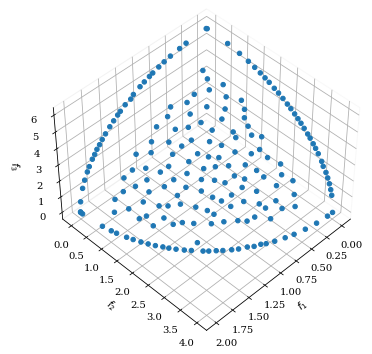
\includegraphics[width=0.3\textwidth]{SMSEMOA_wfg4_hv_3_fp.png}
	\caption{Aproximación al frente de pareto del problema wfg4 con indicador hv usando algoritmoSMSEMOA con 3 objetivos.}
\end{figure}
\clearpage
\begin{figure}
	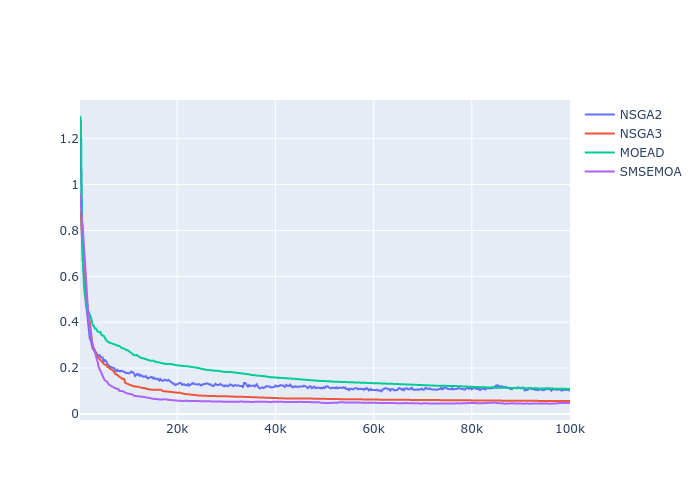
\includegraphics[width=0.3\textwidth]{wfg4_igdp_3_gc.png}
	\caption{Grafico de convergencia del problema wfg4 con indicador igdp con 3 objetivos.}
\end{figure}
\begin{figure}
	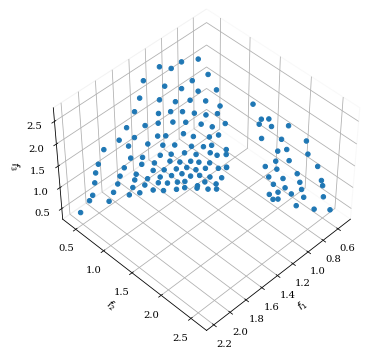
\includegraphics[width=0.3\textwidth]{NSGA3_wfg1_igdp_3_fp.png}
	\caption{Aproximación al frente de pareto del problema wfg1 con indicador igdp usando algoritmoNSGA3 con 3 objetivos.}
\end{figure}
\begin{figure}
	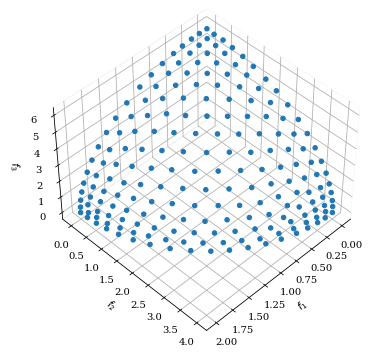
\includegraphics[width=0.3\textwidth]{NSGA3_wfg4_igdp_3_fp.png}
	\caption{Aproximación al frente de pareto del problema wfg4 con indicador igdp usando algoritmoNSGA3 con 3 objetivos.}
\end{figure}
\clearpage
\begin{figure}
	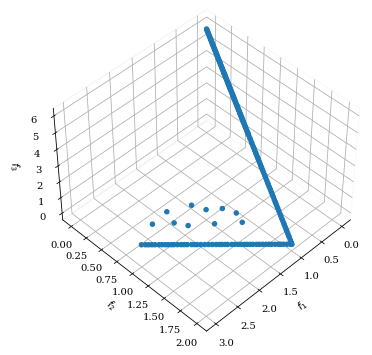
\includegraphics[width=0.3\textwidth]{SMSEMOA_wfg3_igdp_3_fp.png}
	\caption{Aproximación al frente de pareto del problema wfg3 con indicador igdp usando algoritmoSMSEMOA con 3 objetivos.}
\end{figure}
\begin{figure}
	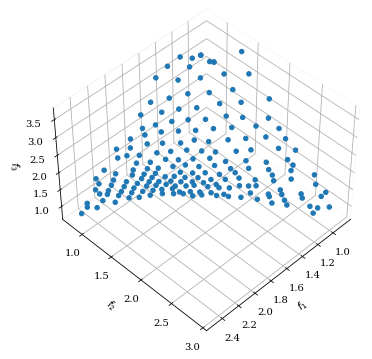
\includegraphics[width=0.3\textwidth]{MOEAD_wfg1_Tiempo_3_fp.png}
	\caption{Aproximación al frente de pareto del problema wfg1 con indicador Tiempo usando algoritmoMOEAD con 3 objetivos.}
\end{figure}
\begin{figure}
	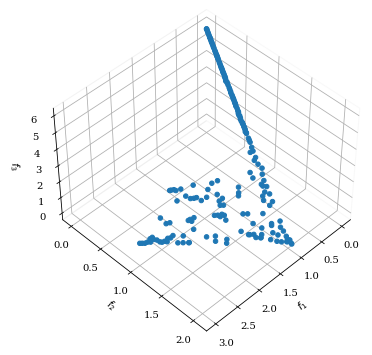
\includegraphics[width=0.3\textwidth]{NSGA2_wfg3_Tiempo_3_fp.png}
	\caption{Aproximación al frente de pareto del problema wfg3 con indicador Tiempo usando algoritmoNSGA2 con 3 objetivos.}
\end{figure}
\clearpage
\begin{figure}
	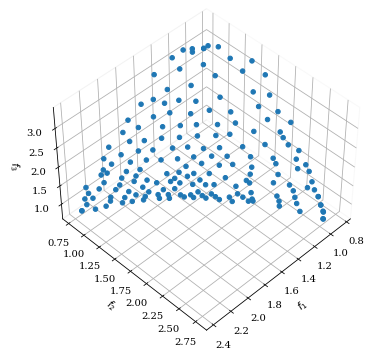
\includegraphics[width=0.3\textwidth]{MOEAD_wfg1_hv_3_fp.png}
	\caption{Aproximación al frente de pareto del problema wfg1 con indicador hv usando algoritmoMOEAD con 3 objetivos.}
\end{figure}
\begin{figure}
	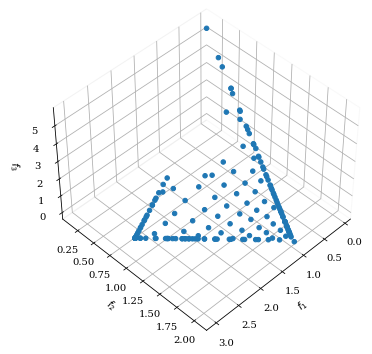
\includegraphics[width=0.3\textwidth]{MOEAD_wfg3_Tiempo_3_fp.png}
	\caption{Aproximación al frente de pareto del problema wfg3 con indicador Tiempo usando algoritmoMOEAD con 3 objetivos.}
\end{figure}
\begin{figure}
	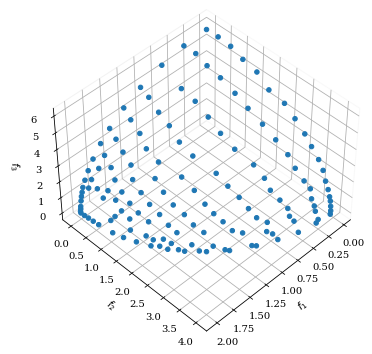
\includegraphics[width=0.3\textwidth]{MOEAD_wfg4_Tiempo_3_fp.png}
	\caption{Aproximación al frente de pareto del problema wfg4 con indicador Tiempo usando algoritmoMOEAD con 3 objetivos.}
\end{figure}
\clearpage
\begin{figure}
	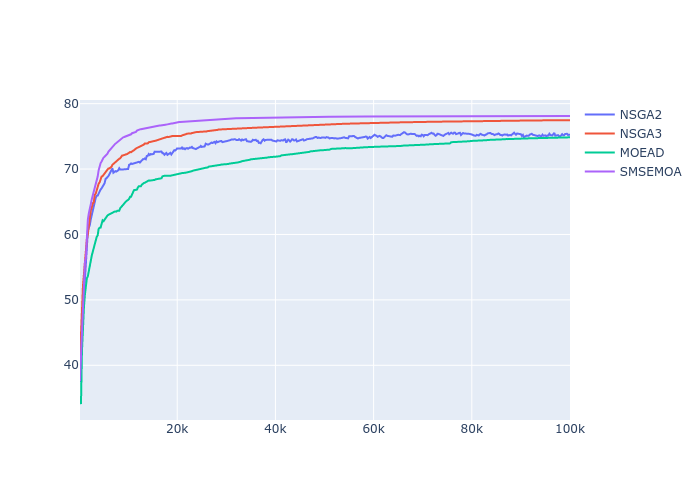
\includegraphics[width=0.3\textwidth]{wfg4_hv_3_gc.png}
	\caption{Grafico de convergencia del problema wfg4 con indicador hv con 3 objetivos.}
\end{figure}
\begin{figure}
	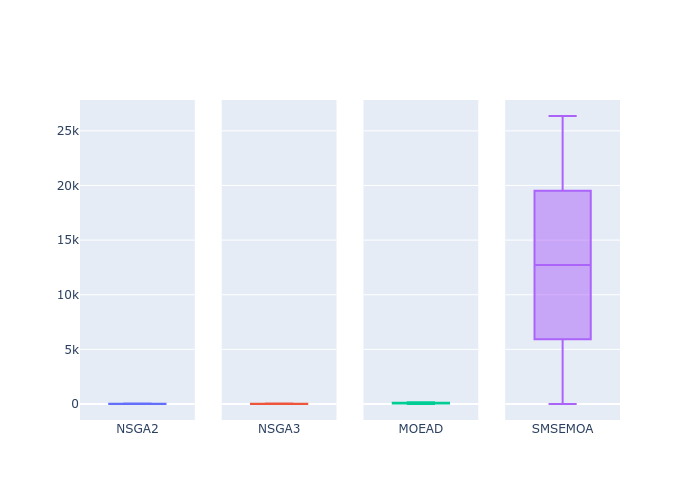
\includegraphics[width=0.3\textwidth]{wfg4_Tiempo_3_bp.png}
	\caption{Diagrama de caja del problema wfg4 con indicador Tiempo con 3 objetivos.}
\end{figure}
\begin{figure}
	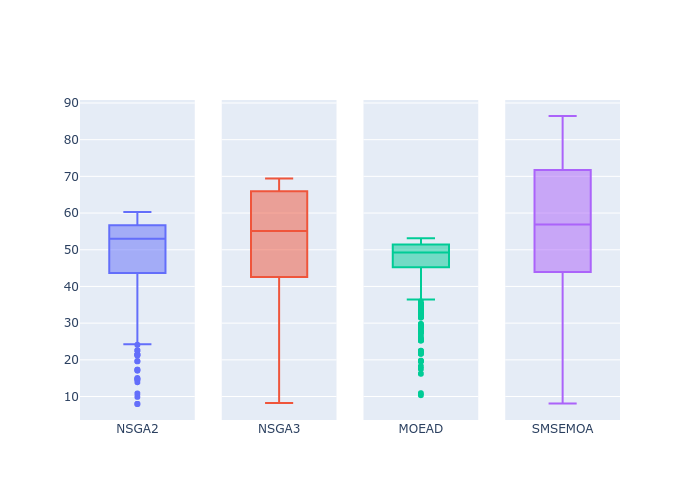
\includegraphics[width=0.3\textwidth]{wfg1_hv_3_bp.png}
	\caption{Diagrama de caja del problema wfg1 con indicador hv con 3 objetivos.}
\end{figure}
\clearpage
\begin{figure}
	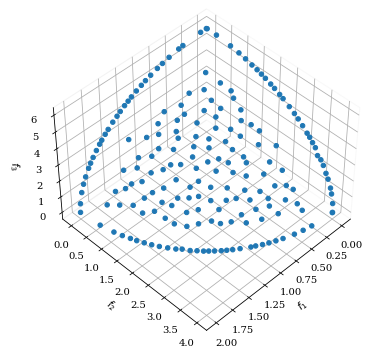
\includegraphics[width=0.3\textwidth]{SMSEMOA_wfg4_Tiempo_3_fp.png}
	\caption{Aproximación al frente de pareto del problema wfg4 con indicador Tiempo usando algoritmoSMSEMOA con 3 objetivos.}
\end{figure}
\begin{figure}
	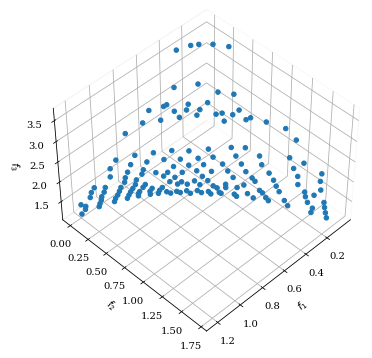
\includegraphics[width=0.3\textwidth]{MOEAD_wfg2_igdp_3_fp.png}
	\caption{Aproximación al frente de pareto del problema wfg2 con indicador igdp usando algoritmoMOEAD con 3 objetivos.}
\end{figure}
\begin{figure}
	\includegraphics[width=0.3\textwidth]{wfg3_igdp_3_gc.png}
	\caption{Grafico de convergencia del problema wfg3 con indicador igdp con 3 objetivos.}
\end{figure}
\clearpage
\begin{figure}
	\includegraphics[width=0.3\textwidth]{MOEAD_wfg4_igdp_3_fp.png}
	\caption{Aproximación al frente de pareto del problema wfg4 con indicador igdp usando algoritmoMOEAD con 3 objetivos.}
\end{figure}
\begin{figure}
	\includegraphics[width=0.3\textwidth]{SMSEMOA_wfg2_hv_3_fp.png}
	\caption{Aproximación al frente de pareto del problema wfg2 con indicador hv usando algoritmoSMSEMOA con 3 objetivos.}
\end{figure}
\begin{figure}
	\includegraphics[width=0.3\textwidth]{MOEAD_wfg1_igdp_3_fp.png}
	\caption{Aproximación al frente de pareto del problema wfg1 con indicador igdp usando algoritmoMOEAD con 3 objetivos.}
\end{figure}
\clearpage
\begin{figure}
	\includegraphics[width=0.3\textwidth]{SMSEMOA_wfg2_Tiempo_3_fp.png}
	\caption{Aproximación al frente de pareto del problema wfg2 con indicador Tiempo usando algoritmoSMSEMOA con 3 objetivos.}
\end{figure}
\begin{figure}
	\includegraphics[width=0.3\textwidth]{wfg4_igdp_3_bp.png}
	\caption{Diagrama de caja del problema wfg4 con indicador igdp con 3 objetivos.}
\end{figure}
\begin{figure}
	\includegraphics[width=0.3\textwidth]{NSGA3_wfg2_Tiempo_3_fp.png}
	\caption{Aproximación al frente de pareto del problema wfg2 con indicador Tiempo usando algoritmoNSGA3 con 3 objetivos.}
\end{figure}
\clearpage
\begin{figure}
	\includegraphics[width=0.3\textwidth]{MOEAD_wfg4_hv_3_fp.png}
	\caption{Aproximación al frente de pareto del problema wfg4 con indicador hv usando algoritmoMOEAD con 3 objetivos.}
\end{figure}
\begin{figure}
	\includegraphics[width=0.3\textwidth]{NSGA3_wfg3_Tiempo_3_fp.png}
	\caption{Aproximación al frente de pareto del problema wfg3 con indicador Tiempo usando algoritmoNSGA3 con 3 objetivos.}
\end{figure}
\begin{figure}
	\includegraphics[width=0.3\textwidth]{NSGA3_wfg2_igdp_3_fp.png}
	\caption{Aproximación al frente de pareto del problema wfg2 con indicador igdp usando algoritmoNSGA3 con 3 objetivos.}
\end{figure}
\clearpage
\begin{figure}
	\includegraphics[width=0.3\textwidth]{NSGA2_wfg2_igdp_3_fp.png}
	\caption{Aproximación al frente de pareto del problema wfg2 con indicador igdp usando algoritmoNSGA2 con 3 objetivos.}
\end{figure}
\begin{figure}
	\includegraphics[width=0.3\textwidth]{wfg1_Tiempo_3_bp.png}
	\caption{Diagrama de caja del problema wfg1 con indicador Tiempo con 3 objetivos.}
\end{figure}
\begin{figure}
	\includegraphics[width=0.3\textwidth]{NSGA3_wfg4_hv_3_fp.png}
	\caption{Aproximación al frente de pareto del problema wfg4 con indicador hv usando algoritmoNSGA3 con 3 objetivos.}
\end{figure}
\clearpage
\begin{figure}
	\includegraphics[width=0.3\textwidth]{wfg2_Tiempo_3_gc.png}
	\caption{Grafico de convergencia del problema wfg2 con indicador Tiempo con 3 objetivos.}
\end{figure}
\begin{figure}
	\includegraphics[width=0.3\textwidth]{SMSEMOA_wfg1_igdp_3_fp.png}
	\caption{Aproximación al frente de pareto del problema wfg1 con indicador igdp usando algoritmoSMSEMOA con 3 objetivos.}
\end{figure}
\begin{figure}
	\includegraphics[width=0.3\textwidth]{MOEAD_wfg2_Tiempo_3_fp.png}
	\caption{Aproximación al frente de pareto del problema wfg2 con indicador Tiempo usando algoritmoMOEAD con 3 objetivos.}
\end{figure}
\clearpage
\begin{figure}
	\includegraphics[width=0.3\textwidth]{NSGA2_wfg4_Tiempo_3_fp.png}
	\caption{Aproximación al frente de pareto del problema wfg4 con indicador Tiempo usando algoritmoNSGA2 con 3 objetivos.}
\end{figure}
\begin{figure}
	\includegraphics[width=0.3\textwidth]{NSGA2_wfg4_hv_3_fp.png}
	\caption{Aproximación al frente de pareto del problema wfg4 con indicador hv usando algoritmoNSGA2 con 3 objetivos.}
\end{figure}
\begin{figure}
	\includegraphics[width=0.3\textwidth]{NSGA2_wfg3_hv_3_fp.png}
	\caption{Aproximación al frente de pareto del problema wfg3 con indicador hv usando algoritmoNSGA2 con 3 objetivos.}
\end{figure}
\clearpage
\begin{figure}
	\includegraphics[width=0.3\textwidth]{wfg3_Tiempo_3_gc.png}
	\caption{Grafico de convergencia del problema wfg3 con indicador Tiempo con 3 objetivos.}
\end{figure}
\begin{figure}
	\includegraphics[width=0.3\textwidth]{wfg4_Tiempo_3_gc.png}
	\caption{Grafico de convergencia del problema wfg4 con indicador Tiempo con 3 objetivos.}
\end{figure}
\begin{figure}
	\includegraphics[width=0.3\textwidth]{NSGA2_wfg1_hv_3_fp.png}
	\caption{Aproximación al frente de pareto del problema wfg1 con indicador hv usando algoritmoNSGA2 con 3 objetivos.}
\end{figure}




\end{document}